\documentclass[11pt,a4paper]{article}

% === Font & encoding (XeLaTeX + xeCJK) ===
\usepackage{fontspec}
\setmainfont{Latin Modern Roman}
\setsansfont{Latin Modern Sans}
\setmonofont{Latin Modern Mono}

% Korean font support via xeCJK (proper spacing between CJK and Latin)
\usepackage{xeCJK}
\setCJKmainfont{Noto Sans CJK KR}[Scale=0.95, BoldFont={Noto Sans CJK KR Bold}]
\setCJKsansfont{Noto Sans CJK KR}[Scale=0.95]
\xeCJKsetup{CJKspace=true, CJKecglue={\hskip 0.15em plus 0.05em}}

% Paragraph formatting for readability
\setlength{\parindent}{1.5em}
\setlength{\parskip}{0.4em plus 0.1em}

% === Layout ===
\usepackage[margin=2cm,headheight=14pt]{geometry}
\usepackage{graphicx}
\usepackage{booktabs}
\usepackage{longtable}
\usepackage{float}
\usepackage{hyperref}
\usepackage{xcolor}
\usepackage{fancyhdr}
\usepackage{titlesec}
\usepackage{caption}
\usepackage{multirow}
\usepackage{enumitem}
\usepackage{array}
\usepackage{tabularx}
\usepackage{amssymb}
\usepackage[normalem]{ulem}

% === Header/Footer ===
\pagestyle{fancy}
\fancyhf{}
\rhead{교차 모델 SAE 분석}
\lhead{LLM 도박 중독}
\cfoot{\thepage}

% === Section styling ===
\titleformat{\section}{\Large\bfseries}{\thesection}{1em}{}
\titleformat{\subsection}{\large\bfseries}{\thesubsection}{1em}{}
\titleformat{\subsubsection}{\normalsize\bfseries}{\thesubsubsection}{1em}{}

% === Hyperlinks ===
\hypersetup{
    colorlinks=true,
    linkcolor=blue!60!black,
    citecolor=green!50!black,
    urlcolor=blue!70!black
}

% === Title ===
\title{\textbf{LLM의 위험 의사결정에 대한\\교차 모델, 교차 도메인 신경 기반 분석}\\[0.3em]
\normalsize ``대형 언어 모델은 도박 중독에 빠질 수 있는가?''}
\author{이승필, 신동현, 이윤정, 김선동\\
\small GIST (광주과학기술원)}
\date{2026년 3월 22일}

\begin{document}
\maketitle
\tableofcontents
\newpage

% ============================================================
% 개요
% ============================================================
\section*{개요}
\addcontentsline{toc}{section}{개요}

대형 언어 모델(Large Language Model)이 도박 과제에서 파산(bankruptcy)할 때---잔고가 0이 될 때까지 반복적으로 배팅을 선택할 때---네트워크 내부에서는 무슨 일이 벌어지는가? 본 보고서는 이러한 내부 ``파산 신호(bankruptcy signal)''가 서로 다른 모델, 도박 도메인, 실험 조건에 걸쳐 공유되는 보편적 속성인지, 아니면 각 설정마다 고유한 신경 패턴을 생성하는지 묻는다.

두 개의 트랜스포머(transformer) 모델을 분석한다: \textbf{Gemma-2-9B-IT} (Google, 42 레이어, 3{,}584차원)와 \textbf{LLaMA-3.1-8B-Instruct} (Meta, 32 레이어, 4{,}096차원). 각 모델은 세 가지 음의 기대값 도박 패러다임---Investment Choice (IC), Slot Machine (SM), Mystery Wheel (MW)---을 수행하여, 6개 모델--패러다임 조합에 걸쳐 총 16{,}000 게임을 생성한다. 배팅 조건(Fixed/Variable)과 프롬프트 구성요소(Goal, Money, Warning, Hint, Persona)를 체계적으로 변화시킨다.

내부 표현(internal representation)을 두 수준에서 검토한다. \textbf{은닉 상태(hidden states)}는 각 트랜스포머 레이어의 전체 활성화 벡터를 포착한다. \textbf{SAE 특성(SAE features)}은 GemmaScope (131K features/layer)와 LlamaScope (32K features/layer)를 통해 추출한 은닉 상태의 희소하고 해석 가능한 분해이다. 분류에는 StandardScaler $\rightarrow$ PCA(50) $\rightarrow$ Logistic Regression (balanced, $C$=1.0)을 사용하며, 5-fold 층화 교차검증(stratified cross-validation)을 적용한다. 200회 순열 검정(permutation test)을 통한 전이 AUC(transfer AUC)로 통계적 유의성을 확인한다.

\textbf{세 가지 연구 질문}:
\begin{itemize}[nosep]
    \item \textbf{RQ1}: Gemma와 LLaMA가 공통적인 파산(BK) 패턴을 공유하는가?
    \item \textbf{RQ2}: 도박 도메인이 바뀌어도 BK 패턴이 유지되는가?
    \item \textbf{RQ3}: 배팅 조건이 바뀌어도 BK 패턴이 유지되는가?
\end{itemize}

\bigskip\hrule\bigskip

% ============================================================
% 핵심 요약
% ============================================================
\section*{핵심 요약}
\addcontentsline{toc}{section}{핵심 요약}

\textbf{RQ1---두 모델 모두 거의 동일한 정확도와 균형 잡힌 신경 구조로 파산을 인코딩한다.} Gemma와 LLaMA는 모든 패러다임에서 BK 분류 AUC가 0.006 이내로 일치한다 (0.954--0.976). L22에서 Gemma는 600개, LLaMA는 1{,}334개의 보편 BK 뉴런(universal BK neuron)을 가지며, 두 모델 모두 촉진(promoting)과 억제(inhibiting) 뉴런의 수가 거의 동일하다. 배팅 유형과 패러다임을 통제한 후에도, SAE 특성의 65--76\%가 BK-유의(permutation $p$=0.000 vs 귀무 ${\sim}$1\%)하다.

\textbf{RQ2---한 도메인에서 학습된 BK 분류기가 다른 도메인의 파산을 예측한다.} Gemma IC$\rightarrow$MW 전이(transfer)는 AUC 0.932 (L18)에 도달하며, LLaMA MW$\rightarrow$IC는 0.805 (L25)에 도달한다. 두 모델 모두 패러다임별 가중치 벡터(weight vector)가 거의 직교(cosine $\approx$ 0.04)함에도 이를 달성하며, 이는 BK 신호가 단일 방향이 아닌 공유된 저차원 부분공간(low-dimensional subspace)을 차지함을 나타낸다.

\textbf{RQ3---Fixed-bet 파산으로 학습된 분류기가 Variable-bet 파산을 예측하며, 그 역도 성립한다.} 교차 배팅 유형 전이(cross-bet-type transfer)는 모든 LLaMA 레이어에서 AUC 0.74--0.93을 보인다 (모두 $p$=0.000). Gemma SAE는 심층 레이어(L30: 0.902)에서 동일 패턴을 확인한다. 415개 SAE 특성이 두 배팅 조건 모두에서 일관된 BK 효과(동일 부호, $d$$\geq$0.3)를 보인다.

\bigskip\hrule\bigskip

% ============================================================
% 1. 실험 설정
% ============================================================
\section{실험 설정}

\subsection{데이터}

\begin{table}[H]
\centering
\caption{데이터셋 개요}
\begin{tabular}{llccc}
\toprule
\textbf{패러다임} & \textbf{모델} & \textbf{게임 수} & \textbf{BK} & \textbf{BK\%} \\
\midrule
IC & Gemma & 1{,}600 & 172 & 10.8\% \\
IC & LLaMA & 1{,}600 & 142 & 8.9\% \\
SM & Gemma & 3{,}200 & 87 & 2.7\% \\
SM & LLaMA & 3{,}200 & 1{,}164 & 36.4\% \\
MW & Gemma & 3{,}200 & 54 & 1.7\% \\
MW & LLaMA & 3{,}200 & 2{,}426 & 75.8\% \\
\bottomrule
\end{tabular}
\end{table}

각 패러다임은 2개의 배팅 유형(Fixed/Variable)과 32개의 프롬프트 조합을 사용한다. IC는 배팅 제약(c10/c30/c50/c70)도 추가로 변화시킨다. SM과 MW에서 LLaMA의 BK 비율은 Gemma보다 13--44배 높으며, 이는 두 모델이 매우 다른 행동 전략을 취하면서도 동등한 정확도로 BK 정보를 인코딩함을 의미한다 (\S\ref{sec:rq1_classification_ko} 참조).

\subsection{핵심 정의}

\begin{description}[style=nextline, leftmargin=2em]
    \item[파산 (Bankruptcy, BK)] 누적 손실로 잔고가 \$0에 도달한 상태. 주요 결과 변수(outcome variable).
    \item[의사결정 지점 (Decision Point, DP)] 각 게임에서 모델의 마지막 배팅/정지 결정 시점의 활성화 상태.
    \item[보편 BK 뉴런 (Universal BK neuron)] 테스트된 모든 패러다임에서 BK 결과와의 상관이 FDR-유의(BH, $p$<0.01)하며 부호가 동일한 뉴런.
    \item[교차 도메인 전이 (Cross-domain transfer)] 한 패러다임에서 BK 분류기를 학습하고 다른 패러다임에서 테스트. AUC $\gg$ 0.5이며 순열 $p$<0.05이면 공유된 BK 구조를 나타냄.
    \item[교차 배팅 유형 전이 (Cross-bet-type transfer, F1)] Fixed-bet 게임에서 BK 분류기를 학습하고 Variable-bet 게임에서 테스트 (및 그 역).
\end{description}

\bigskip\hrule\bigskip

% ============================================================
% 2. RQ1
% ============================================================
\section{RQ1: 두 모델이 공통적인 BK 패턴을 공유하는가?}

\subsection{BK 분류}\label{sec:rq1_classification_ko}

두 모델 모두 각 최적 레이어에서 세 패러다임 전부에서 BK 분류 AUC > 0.95를 달성한다.

\begin{table}[H]
\centering
\caption{BK 분류 AUC}
\begin{tabular}{lccc}
\toprule
\textbf{패러다임} & \textbf{Gemma} & \textbf{LLaMA} & \textbf{차이} \\
\midrule
SM & 0.976 (L20) & 0.974 (L8) & 0.002 \\
IC & 0.960 (L30) & 0.954 (L12) & 0.006 \\
MW & 0.966 (L30) & 0.963 (L16) & 0.003 \\
\bottomrule
\end{tabular}
\end{table}

두 모델은 서로 다른 깊이에서 최고점을 보인다---Gemma는 L20--L30, LLaMA는 L8--L16---그러나 최적 AUC 값의 차이는 최대 0.006이다. LLaMA MW의 BK 비율(75.8\%)이 Gemma MW(1.7\%)보다 44배 높음에도 이러한 결과가 유지된다. 분류 파이프라인이 균형 클래스 가중치(balanced class weights)를 사용하므로, 이 동등성은 기저율(base rate)의 산물이 아니다. BK 정보는 두 아키텍처 모두에서 동등한 충실도(fidelity)로 존재한다.

\subsection{보편 BK 뉴런}

\begin{table}[H]
\centering
\caption{보편 BK 뉴런 (L22)}
\begin{tabular}{lcc}
\toprule
 & \textbf{Gemma (3-패러다임)} & \textbf{LLaMA (2-패러다임)} \\
\midrule
전체 뉴런 수 & 3{,}584 & 4{,}096 \\
보편 BK 뉴런 & 600 (16.7\%) & 1{,}334 (32.6\%) \\
촉진 / 억제 & 302 / 298 & 672 / 662 \\
\bottomrule
\end{tabular}
\end{table}

LLaMA의 높은 수치는 주로 우연 기준선(chance baseline)의 차이를 반영한다: 2-패러다임 부호 일관성의 우연 기준선은 50\%인 반면, 3-패러다임은 25\%이다. 핵심 발견은 절대 수치가 아니라 \textbf{균형 비율}이다: 두 모델 모두 테스트된 모든 레이어(L8--L30)에서 거의 동일한 수의 촉진 뉴런과 억제 뉴런을 통해 BK를 인코딩한다. 이러한 양방향 구조는 BK-촉진 신호와 BK-억제 신호가 공존하는 ``밀고-당기기(push-pull)'' 메커니즘을 시사한다.

\subsection{요인 분해}

각 SAE 특성에 대해 OLS 회귀(\texttt{feature $\sim$ outcome + bet\_type + paradigm})를 수행하여, 배팅 유형과 패러다임을 통제한 후 BK 결과가 독립적으로 기여하는지 검증한다.

\begin{table}[H]
\centering
\caption{결과-유의 특성}
\begin{tabular}{lcccc}
\toprule
\textbf{모델} & \textbf{패러다임} & \textbf{특성 수} & \textbf{결과-유의} & \textbf{순열 귀무} \\
\midrule
Gemma & IC+SM+MW & 581 & 65.2\% (379) & ${\sim}$1\% \\
LLaMA & IC+SM & 1{,}418 & 69.5\% (985) & ${\sim}$1\% \\
LLaMA & IC+SM+MW & 1{,}056 & 75.8\% (800) & ${\sim}$1\% \\
\bottomrule
\end{tabular}
\end{table}

LLaMA 내에서, MW를 세 번째 패러다임으로 추가하면 결과-유의 비율이 69.5\%에서 75.8\%로 증가하며, 이는 추가 도메인이 패러다임 특이적 잡음을 필터링하되 BK 신호를 희석하지 않음을 나타낸다. 세 분해 모두 순열 귀무(${\sim}$1\%)를 60배 이상 초과한다.

\begin{figure}[H]
\centering
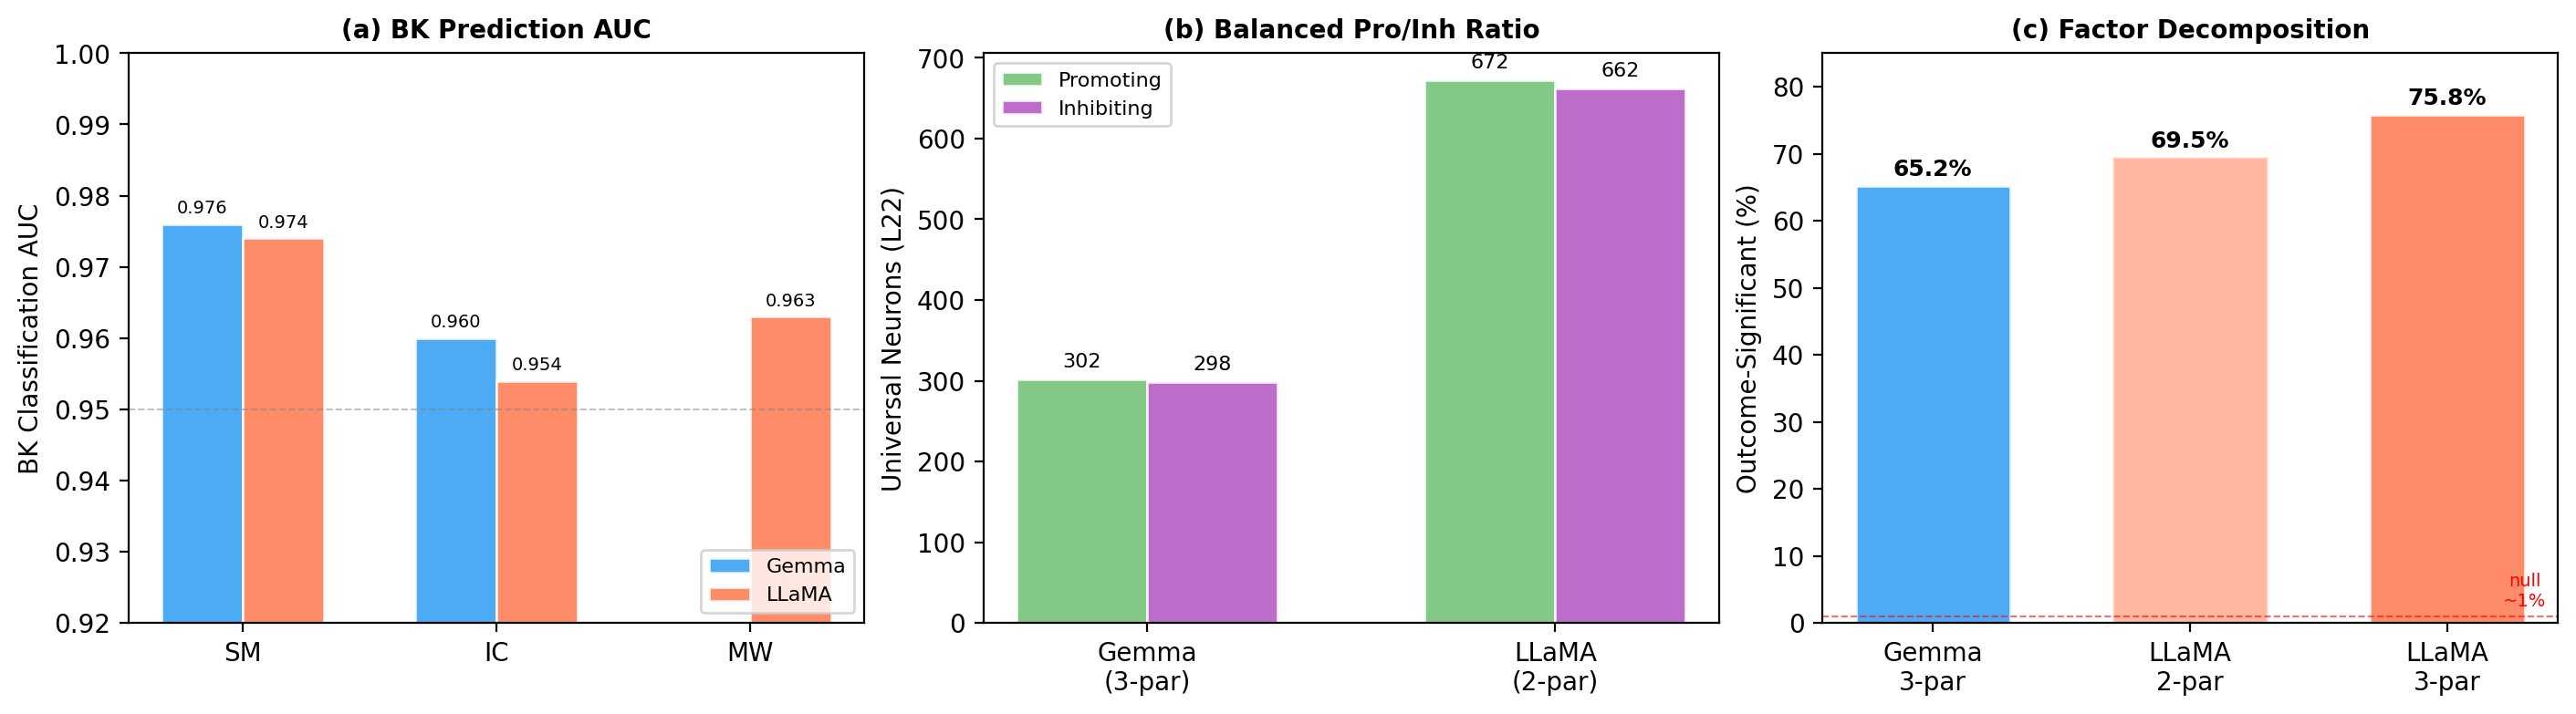
\includegraphics[width=\textwidth]{figures/v10_fig1_rq1_overview.png}
\caption{(a) 교차 모델 BK 분류 AUC. (b) 보편 BK 뉴런: 균형 잡힌 촉진/억제 비율. (c) 요인 분해: 65--76\% 결과-유의 vs ${\sim}$1\% 귀무.}
\label{fig:rq1_overview_ko}
\end{figure}

\subsection{RQ1 요약}

BK 예측 정확도는 아키텍처 간 동등하다 (AUC 차이 $\leq$ 0.006). 두 모델 모두 균형 잡힌 촉진/억제 뉴런 구조를 유지한다. SAE 특성의 65--76\%가 교란 변수와 독립적으로 BK를 인코딩한다. 이 세 관찰은 서로 다른 훈련 데이터와 모델 크기에도 불구하고 두 아키텍처에서 공유된 BK 표현(shared BK representation)이 발생함과 일치한다.

\bigskip\hrule\bigskip

% ============================================================
% 3. RQ2
% ============================================================
\section{RQ2: 도메인이 바뀌어도 BK 패턴이 유지되는가?}

\subsection{교차 도메인 전이}

\begin{table}[H]
\centering
\caption{Gemma SAE 전이 (최적 레이어)}
\begin{tabular}{lcc}
\toprule
\textbf{전이} & \textbf{AUC} & \textbf{$p$} \\
\midrule
IC $\rightarrow$ MW & 0.932 & 0.000 \\
IC $\rightarrow$ SM & 0.913 & 0.000 \\
SM $\rightarrow$ MW & 0.867 & 0.000 \\
MW $\rightarrow$ IC & 0.853 & 0.000 \\
SM $\rightarrow$ IC & 0.646 & 0.000 \\
\bottomrule
\end{tabular}
\end{table}

\begin{table}[H]
\centering
\caption{LLaMA 3-패러다임 전이 (최적 레이어)}
\begin{tabular}{lcc}
\toprule
\textbf{전이} & \textbf{AUC} & \textbf{$p$} \\
\midrule
MW $\rightarrow$ IC & 0.805 & 0.000 \\
SM $\rightarrow$ IC & 0.749 & 0.000 \\
IC $\rightarrow$ MW & 0.680 & 0.000 \\
MW $\rightarrow$ SM & 0.682 & 0.000 \\
IC $\rightarrow$ SM & 0.577 & 0.000 \\
\bottomrule
\end{tabular}
\end{table}

두 모델 모두 MW를 포함하는 전이에서 강한 성능을 보이며 (AUC 0.68--0.93), IC$\leftrightarrow$SM 전이는 상대적으로 약하고 레이어에 따라 달라진다. MW는 ``허브(hub)'' 패러다임으로 기능한다: MW에서 학습되거나 MW에 적용된 BK 패턴이 다른 도메인으로 잘 전이된다.

\begin{figure}[H]
\centering
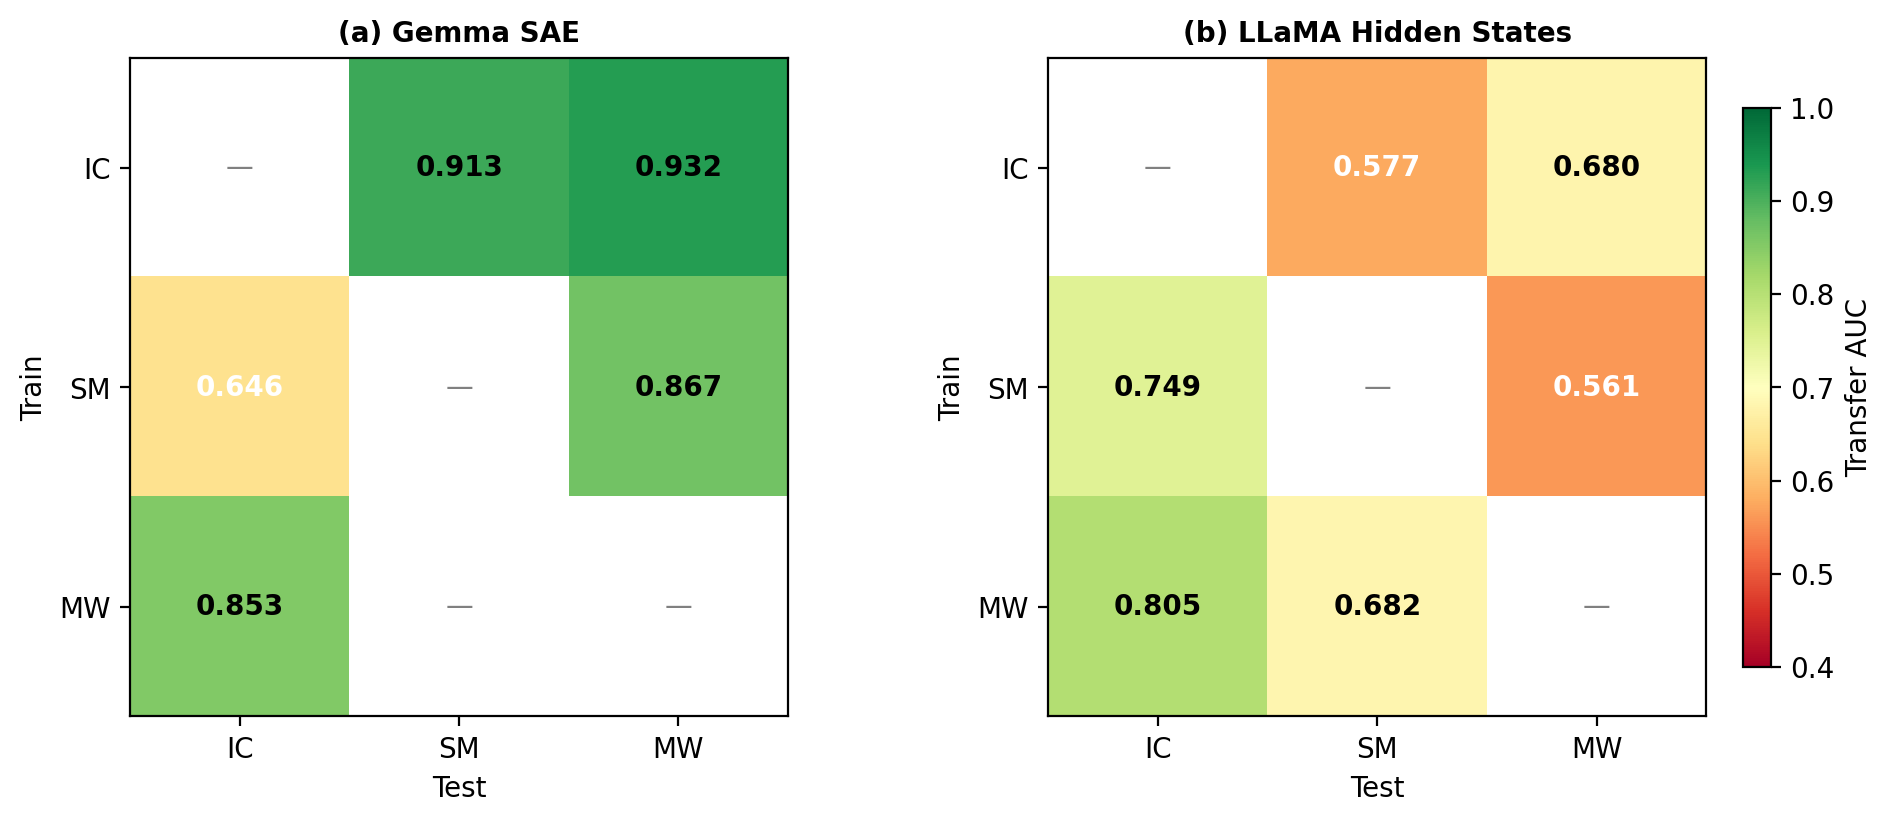
\includegraphics[width=\textwidth]{figures/v10_fig2_rq2_transfer.png}
\caption{교차 도메인 전이 히트맵. (a) Gemma SAE. (b) LLaMA hidden states. 녹색 = 높은 전이; 노란색/빨간색 = 약한 전이.}
\label{fig:rq2_transfer_ko}
\end{figure}

\subsection{공유 BK 부분공간}

패러다임별 분류기의 가중치 벡터가 거의 직교(cosine $\approx$ 0.04)함에도, 이 가중치 벡터들에 대한 PCA로 추출한 저차원 부분공간(low-dimensional subspace)이 높은 AUC를 달성한다.

\begin{table}[H]
\centering
\caption{공유 부분공간 성능}
\begin{tabular}{lcc}
\toprule
 & \textbf{Gemma (3D)} & \textbf{LLaMA (2D)} \\
\midrule
IC AUC & 0.862 & 0.901 \\
SM AUC & 0.899 & 0.943 \\
MW AUC & 0.970 & --- \\
가중치 코사인 & ${\sim}$0.04 & 0.038 \\
\bottomrule
\end{tabular}
\end{table}

거의 직교하는 가중치 벡터에서 높은 부분공간 AUC가 나온다는 것은, BK 신호가 단일 축에 집중되지 않고 다차원 부분공간에 분산되어 있음을 의미한다.

\subsection{Hidden States vs SAE 전이 비교}

Hidden states가 대부분의 교차 도메인 전이 방향에서 SAE보다 우수하다 (Gemma IC$\rightarrow$SM: +0.247; SM$\rightarrow$MW: +0.101; LLaMA SM$\rightarrow$IC: +0.064). SAE 희소화(sparsification)가 교차 도메인 일관성을 상실할 수 있으며, 이는 BK 신호가 부분적으로 희소 분해가 폐기하는 분산적이고 낮은 크기의 활성화에 의존함을 시사한다.

\subsection{RQ2 요약}

교차 도메인 전이가 두 모델 모두에서 성공한다 (AUC 0.58--0.93, 모두 $p$=0.000). MW가 가장 강한 허브 패러다임이다. 직교 가중치 벡터에도 불구하고 공유 저차원 부분공간이 BK를 포착한다. BK 인코딩은 심층 레이어에서 도박 도메인 간에 일반화된다.

\bigskip\hrule\bigskip

% ============================================================
% 4. RQ3
% ============================================================
\section{RQ3: 배팅 조건이 바뀌어도 BK 패턴이 유지되는가?}

\subsection{교차 배팅 유형 전이 (F1)}

Fixed-bet 게임에서만 학습된 BK 분류기를 Variable-bet 게임에 적용하며, 그 역도 수행한다.

\begin{table}[H]
\centering
\caption{LLaMA IC Hidden State 전이}
\begin{tabular}{lccc}
\toprule
\textbf{레이어} & \textbf{Fix$\rightarrow$Var AUC} & \textbf{Var$\rightarrow$Fix AUC} & \textbf{Both $p$} \\
\midrule
L8 & 0.872 & 0.842 & 0.000 \\
L12 & 0.772 & 0.927 & 0.000 \\
L22 & 0.736 & 0.912 & 0.000 \\
L30 & 0.819 & 0.911 & 0.000 \\
\bottomrule
\end{tabular}
\end{table}

\begin{table}[H]
\centering
\caption{Gemma IC SAE 전이}
\begin{tabular}{lccc}
\toprule
\textbf{레이어} & \textbf{Fix$\rightarrow$Var AUC} & \textbf{Var$\rightarrow$Fix AUC} & \textbf{Both $p$} \\
\midrule
L18 & 0.808 & 0.726 & 0.000 \\
L30 & 0.902 & 0.696 & 0.000 \\
L10 & NS & NS & --- \\
\bottomrule
\end{tabular}
\end{table}

LLaMA에서는 모든 레이어와 양방향 모두 $p$=0.000을 보인다. Var$\rightarrow$Fix 전이(0.84--0.93)가 Fix$\rightarrow$Var(0.74--0.87)보다 일관되게 강한데, 이는 Variable 게임이 Fixed BK 영역을 포괄하는 더 넓은 활성화 공간을 탐색하기 때문일 수 있다. Gemma에서는 심층 레이어가 성공하나(L30: Fix$\rightarrow$Var 0.902) 얕은 레이어(L10)는 실패하며---이는 교차 조건 전이에 심층 표현이 필요하다는 일반적 패턴과 일치한다. Gemma IC는 Variable BK 사례가 14건에 불과하여, Gemma 특이적 배팅 유형 분석의 통계적 검정력(statistical power)이 제한됨에 유의한다.

\begin{figure}[H]
\centering
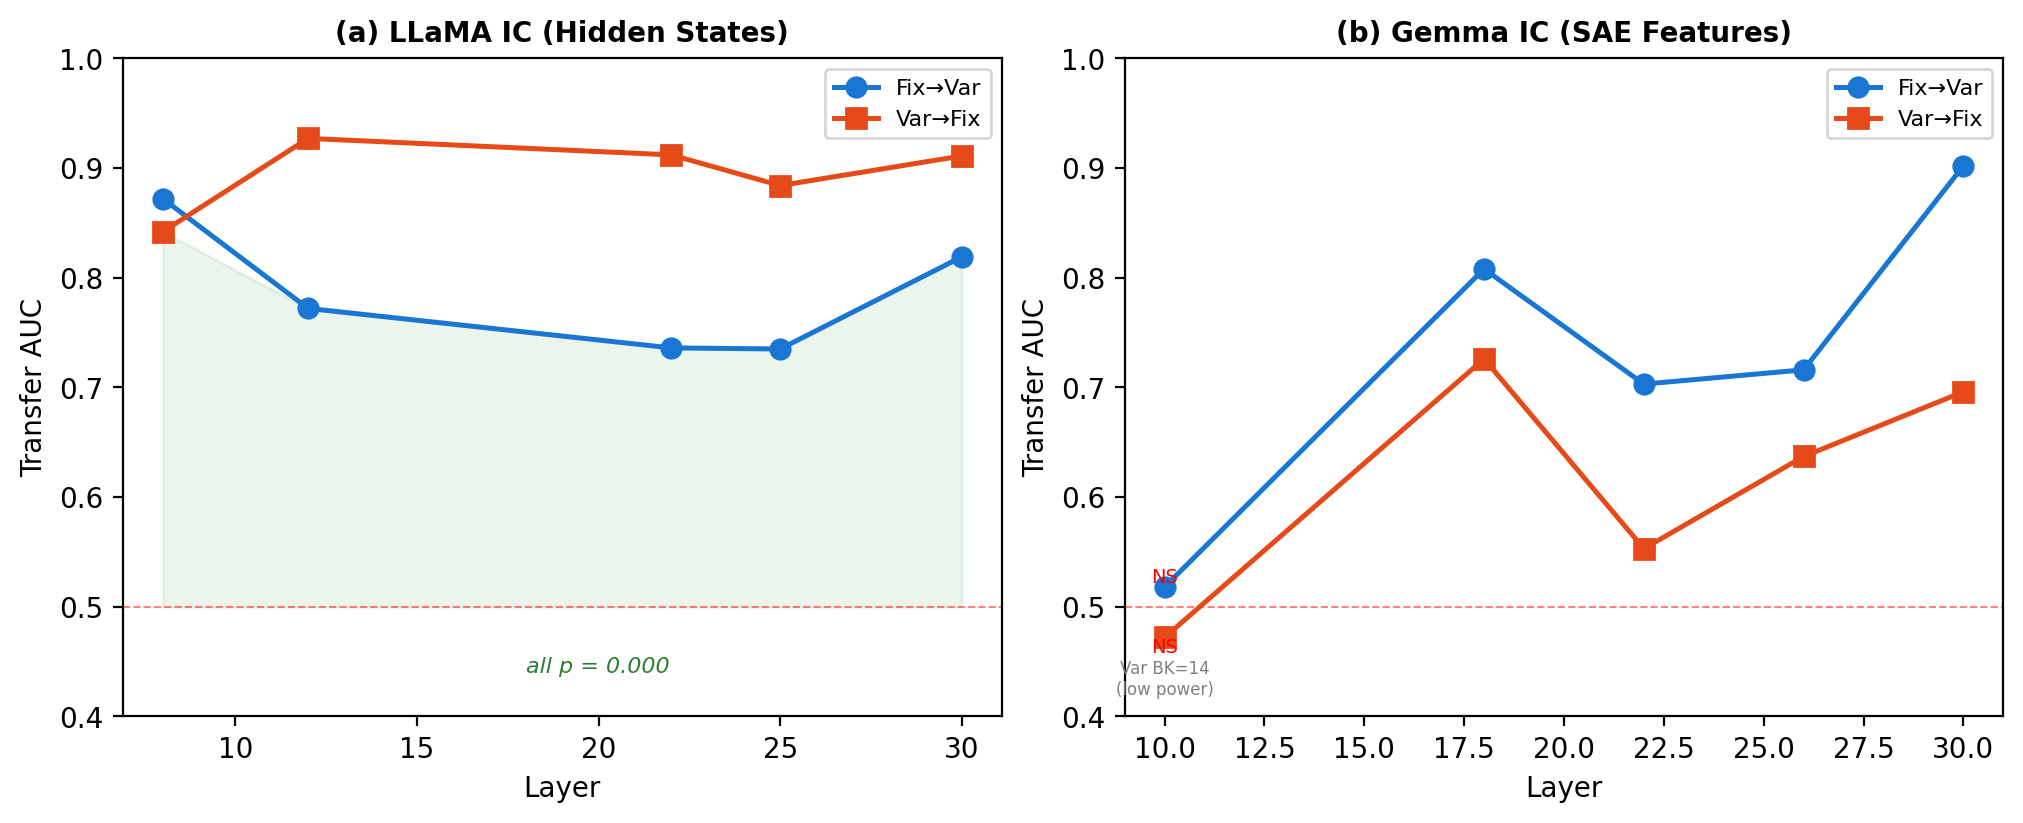
\includegraphics[width=\textwidth]{figures/v10_fig3_rq3_bettype_transfer.png}
\caption{교차 배팅 유형 전이. (a) LLaMA: 모든 레이어, 양방향, 모두 $p$=0.000. (b) Gemma SAE: 심층 레이어 성공; L10 실패.}
\label{fig:rq3_bettype_ko}
\end{figure}

\subsection{방향 코사인 및 공통 특성}

Variable BK 방향과 Fixed BK 방향 사이의 코사인 유사도(cosine similarity)가 보완적 증거를 제공한다. LLaMA IC는 모든 hidden state 레이어에서 $\cos > 0.81$, SAE 수준에서 $\cos$ 0.77--0.85를 보인다. Gemma IC는 얕은 레이어에서 음의 값으로 시작하여 L30에서 $\cos$ ${\sim}$0.39로 수렴하며---Variable BK 표본 크기($n$=14)로 인해 약하다.

SAE L22에서 415개 LLaMA 특성(및 35개 Gemma 특성)이 두 배팅 조건 모두에서 $d$$\geq$0.3이며 동일 부호를 보인다. 균형 잡힌 촉진/억제 비율(LLaMA: 213/202)은 \S2.2의 보편 뉴런 구조를 반영한다.

\begin{figure}[H]
\centering
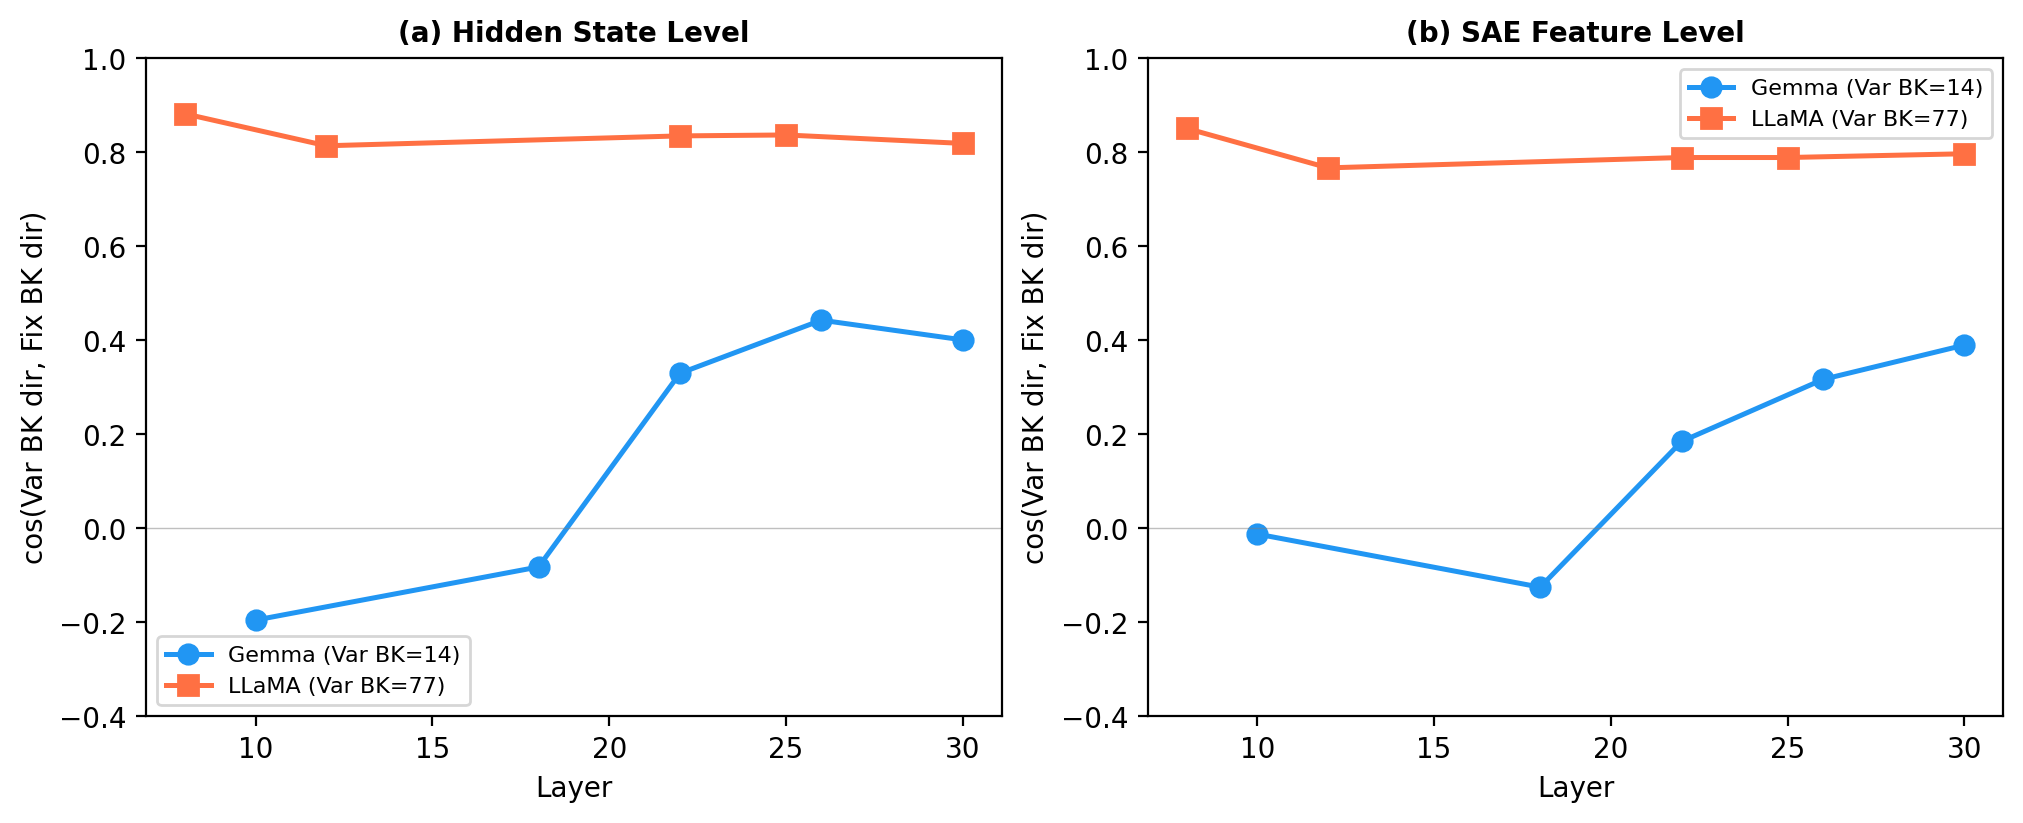
\includegraphics[width=\textwidth]{figures/v10_fig4_rq3_direction_cosine.png}
\caption{Var/Fix 방향 코사인. (a) hidden state 수준. (b) SAE 수준. LLaMA $\cos$>0.77 전 레이어; Gemma는 심층에서 수렴.}
\label{fig:rq3_cosine_ko}
\end{figure}

\subsection{G-프롬프트 및 배팅 제약 효과}

G (Goal-setting) 프롬프트는 두 모델 모두에서 활성화를 BK 방향으로 이동시킨다 (Gemma SM에서 $\cos$ = +0.85, LLaMA SM에서 L22 기준 +0.63). 배팅 제약(c10$\rightarrow$c70)은 BK 확률에 선형적으로 대응한다 (Gemma $r$=0.979, LLaMA $r$=0.987; 단, $n$=4 데이터 포인트로 이 선형 주장의 강도가 제한됨에 유의). 이러한 관찰은 BK 표현이 이진적 BK/Safe 구분이 아닌 연속적 위험 크기(continuous risk magnitude)를 인코딩함을 시사한다.

\subsection{RQ3 요약}

F1 교차 배팅 유형 전이 분석은 Fixed와 Variable 배팅 조건이 심층 레이어에서 동일한 기저 BK 표현을 공유한다는 직접적 증거를 제공한다. 방향 코사인, 공통 특성, G-프롬프트 정렬이 모두 같은 방향을 가리킨다. BK 인코딩은 두 모델 모두에서 Fixed/Variable 조작에 대해 강건하다.

\bigskip\hrule\bigskip

% ============================================================
% 5. NMT 논문 §3.2에 대한 함의
% ============================================================
\section{NMT 논문 \S3.2에 대한 함의}

논문의 \S3.2는 활성화 패칭(activation patching)을 통해 LLaMA SM에서 112개의 인과적 특성(causal features)을 식별하며, 안전 특성(safe features)은 L4--L19에, 위험 특성(risky features)은 L24+에 위치한다. 본 분석은 해당 단일 모델, 단일 도메인 발견을 세 방향으로 확장한다:

\textbf{교차 모델(Cross-model)}: Gemma는 거의 동일한 BK 분류 성능(0.976 vs 0.974)과 동일한 균형 촉진/억제 뉴런 구조를 보인다. 112개 인과적 특성은 LLaMA 특이적 산물이 아니라 두 아키텍처 모두에 존재하는 속성을 반영할 가능성이 높다.

\textbf{교차 도메인(Cross-domain)}: BK 분류기가 IC, SM, MW 간에 AUC 최대 0.932로 전이된다. 요인 분해는 특성의 65--76\%가 패러다임과 독립적으로 BK를 인코딩함을 보인다. SM에서 식별된 인과적 특성은 다른 도박 도메인으로 일반화될 가능성이 높다.

\textbf{교차 조건(Cross-condition)}: 교차 배팅 유형 전이(AUC 0.74--0.93)는 BK 표현이 Fixed/Variable 조작에 강건함을 입증한다---이는 논문의 핵심 행동 발견(Variable 배팅이 파산을 증가시킴)을 생성하는 바로 그 조작이다. 행동 결과가 분기하는 가운데서도 신경 표현은 안정적으로 유지된다.

\bigskip\hrule\bigskip

% ============================================================
% 6. 한계
% ============================================================
\section{한계}

\begin{enumerate}[leftmargin=2em]
    \item \textbf{상관적 증거만 존재.} 본 보고서의 모든 분석은 상관적(correlational)이다. 활성화 패칭을 통한 인과적 검증은 LLaMA SM(논문 \S3.2)에서만 수행되었다. 교차 모델 및 교차 도메인 인과 검증은 보류 중이다.

    \item \textbf{표본 크기 불균형.} Gemma IC는 Variable BK 사례가 14건에 불과하여, Gemma 배팅 유형 분석의 검정력이 심각하게 제한된다. Gemma MW는 54건의 BK를 가진다. LLaMA MW는 2{,}426건 BK(75.8\%)---이 높은 기저율에서는 사소한 분류기도 좋은 성능을 보인다; 균형 클래스 가중치가 부분적으로 완화하지만, 보완적 지표(balanced accuracy, F1)가 주장을 강화할 것이다.

    \item \textbf{레이어 범위.} LLaMA hidden states는 5개 레이어(L8, L12, L22, L25, L30)에서 추출되며 전체 32개가 아니다. 이 체크포인트 사이의 레이어 특이적 현상이 누락될 수 있다.

    \item \textbf{배팅 제약 선형성.} $r$=0.979/0.987 선형 매핑은 4개 데이터 포인트(c10, c30, c50, c70)에서만 계산된다. $df$=2이므로, 무작위 관계도 빈번하게 선형으로 나타날 수 있다.

    \item \textbf{공통 BK 특성.} 415개 공통 특성(두 배팅 유형 모두에서 $d$$\geq$0.3, 동일 부호)은 순열 귀무(permutation null) 비교가 없다. 이 기준을 우연히 충족하는 특성의 기대 수가 계산되지 않았다.

    \item \textbf{다중 비교.} FDR 보정은 개별 분석 내에서 적용되지만 전체 분석 세트에 걸쳐서는 적용되지 않는다. 효과 크기(effect size)를 일차적 증거로 다루어야 한다.

    \item \textbf{두 모델만 분석.} 다른 아키텍처(예: Qwen, Mistral)로의 일반화는 검증되지 않았다.
\end{enumerate}

\bigskip\hrule\bigskip

% ============================================================
% 7. 다음 단계
% ============================================================
\section{다음 단계}

\begin{enumerate}[leftmargin=2em]
    \item \textbf{Gemma 활성화 패칭}: Gemma의 600개 보편 BK 뉴런이 BK 결과에 인과적으로 영향을 미치는지 검증하여, 교차 모델 인과적 일반화를 확인한다.
    \item \textbf{IC/MW 활성화 패칭}: SM에서 식별된 인과적 특성을 다른 패러다임에서 검증한다.
    \item \textbf{공통 특성에 대한 순열 귀무}: 레이블 순열 하에서 두 배팅 유형 모두 $d$$\geq$0.3을 충족하는 특성의 기대 수를 계산한다.
    \item \textbf{고-BK 조건에 대한 balanced accuracy}: LLaMA MW(75.8\% BK)에 대해 AUC와 함께 balanced accuracy 및 F1을 보고한다.
    \item \textbf{G-프롬프트 메커니즘}: 유사한 방향 정렬에도 불구하고 존재하는 16배 행동 격차(Gemma G: 20.75배 vs LLaMA G: 1.26배)를 조사한다.
\end{enumerate}

\end{document}
